\chapter{Testing}

Testing is crucial to verifying software. The team decided to take a multi-pronged approach towards testing, focusing on client feedback, visual testing, and code testing. By splitting up testing in such a manner, testing is done both informally and formally, covering the entire system from the ground up. Client feedback is crucial, and it is here that this section will start.

\section{Client Feedback}

Ultimately, client feedback is the most significant metric of success. Completing this project would be meaningless if it went against the clients wishes. Because of this approach, the team kept the client in the loop, ensuring that the team never deviated far from the client's desires. Table \ref{stats} quantifies interactions with the client. Throughout the project, the team revived feedback from the client, both good and bad, with changes made to keep the project on the right track.

\begin{table}[H]
\centering
\begin{tabular}{|l|l|}
\hline
\textbf{Number of Skype meetings}        & 4  \\ \hline
\textbf{Number of face to face meetings} & 1  \\ \hline
\textbf{Number of emails exchanged}      & 57 \\ \hline
\end{tabular}
\caption{Client interaction statistics}
\label{stats}
\end{table}

Ultimately, the client was happy with the project and the progress made. They received a copy of final report, and all the code created in the course of the project. It was a pleasure working with the client, and the team wishes them future success with oneTRANSPORT and the oneM2M standard.

\section{Visual Testing}

The purpose of these tests was to show the client data federation, and video streaming capabilities in action. Many tools were used including platform integrated tools, third party applications or self-developed visual testing platforms. By using a wide variety of tools to test, correctness is checked on many levels, increasing the team's confidence in the final product.

\subsection{Eclipse OM2M}

\begin{figure}[H]
  \centering
  \frame{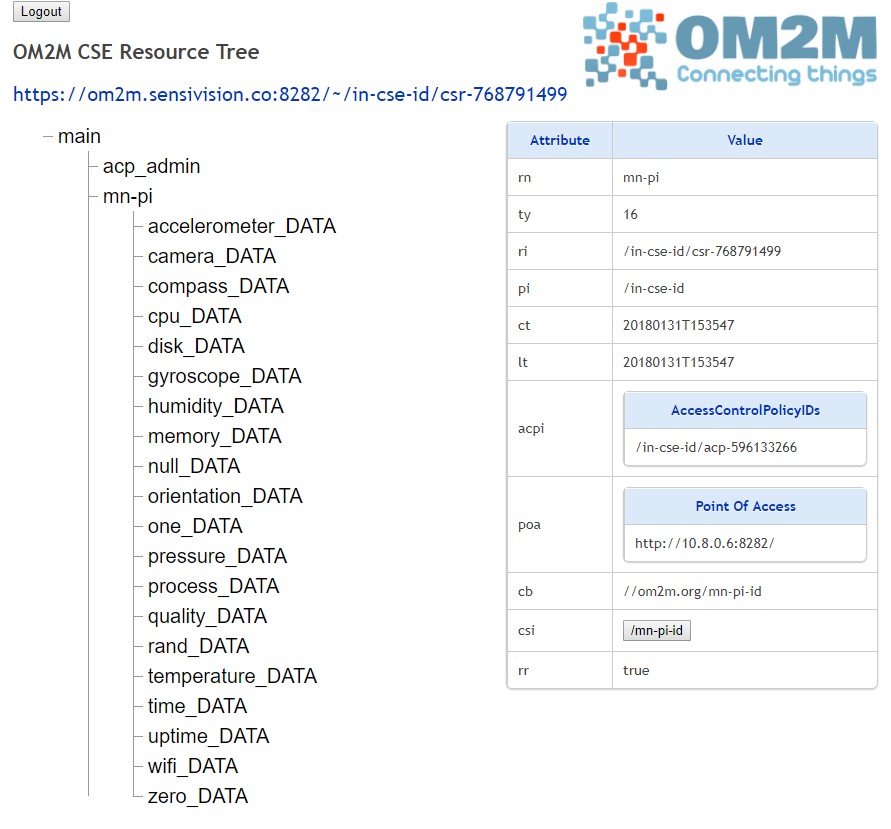
\includegraphics[width=.6\linewidth]{INdata}}
  \caption{Eclipse OM2M CSE Resource Tree}
  \label{fig:viewing-the-eclipse-resource-tree}
\end{figure}

Eclipse OM2M is packaged with an interactive resource tree visualiser, that runs on each device. This interface was used to first experiment with the sample lamp plug-in after installing it, and then to aid in forming an understanding of how the overall OM2M set-up functioned. Once the plug-in was developed and ready to test, it was compiled and copied to the Raspberry Pi. However, the MN configuration files had to be altered before it could be properly run.

Initially, it did not fully work, so by using the interface the team began testing and narrowing down bugs. After some time, the plug-in was feature complete, with each feature fully tested and verified working.

This interface, while not crucial, was very helpful in development as it significantly simplified the development process. Without it, the team would have needed to research and use a third-part oneM2M client, or resort to a REST API client, and OM2M exposes and extends a powerful RESTful API. For example, if a method to create an AE was not working correctly, it would be absent from the interface and if the server's ID was changed, it would be shown in the interface under CSI.

\subsection{OpenMTC}

Unlike Eclipse OM2M, OpenMTC does not provide a native resource tree visualiser, and only serves a RESTful API. If the team had started off using OpenMTC instead of OM2M, it would likely have been necessary to research and use a third-party client. However, by this stage of the project, the team had formed a good understanding of how oneM2M functioned, and how to use it. As a result, the RESTful API was sufficient for testing and validating OpenMTC.

\begin{figure}[H]
  \centering
  \frame{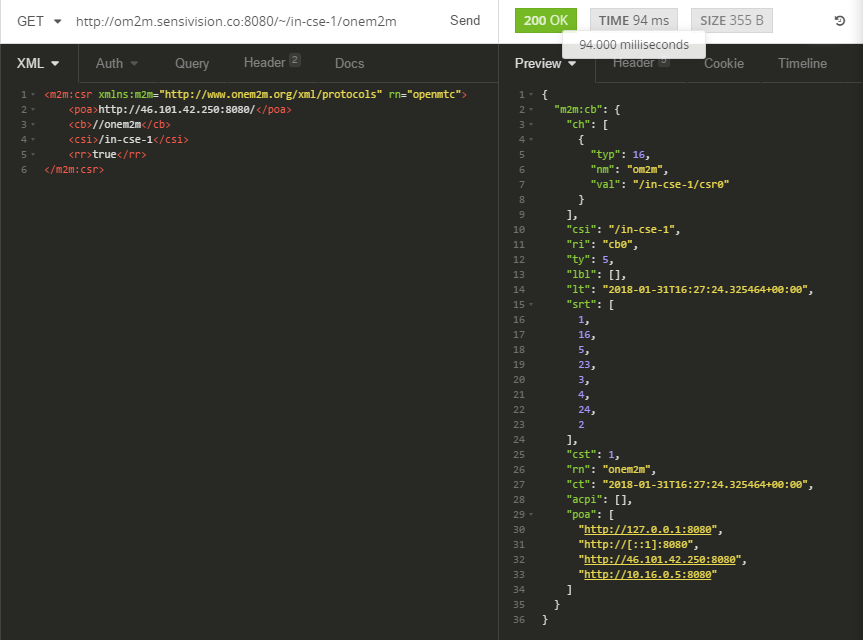
\includegraphics[width=.6\linewidth]{insomnia}}
  \caption{The Insomnia REST client}
  \label{fig:insomnia-rest-client}
\end{figure}

Now to verify the plug-in, a third-party REST client by the name of Insomnia was used to create and run queries to verify the resources and data containing inside the OpenMTC system. Using Insomnia, each sensor was checked in turn and validated, checking streaming worked as expected. Overall this was a success, with the Python OpenMTC having significantly higher performance than Java OM2M. This could be due to either the overhead of the Java Virtual Machine being much greater than the Python runtime environment, and better software engineering.

\subsection{Video Streaming}

To measure the relative performance of the camera streams in both OM2M and OpenMTC, a visualization web application was developed. This web application consisted of two major parts:

\begin{itemize}
\item A PHP based oneM2M Proxy that would retrieve the last video frame on the client's behalf. This is necessary as JavaScript only supports relatively few protocols, and oneM2M is unfortunately not one of them.
\item A web page served by NGINX with JavaScript to poll for the latest frame, decode the base64 into a JPEG image, and display it to the client, with CSS to make the web page look professional.
\item While not technically part of the system, a modern web browser was used to view the web page.
\end{itemize}

This web application was publicly hosted in the Digital Ocean droplet, and then shared with the client. The different platforms were demonstrated and compared to identify the best performing solution. Ultimately while OM2M could broadcast roughly 5 frames per second, OpenMTC could broadcast roughly 20 frames per second with this set-up.

\section{Code Testing}

While visual testing is important, code testing is of at least equal importance. This section will describe the methods used.

\subsection{Pair Programming}

In critical sections of the project, pair programming was used to help quickly and safely develop the product with the insight of multiple team members. This was very useful as it allowed the team to discuss approaches and arrive at the correct one with less trial and error.

However, as the project progressed past such critical sections, pair programming was discontinued in favour of individual work, as it would have produced diminishing returns.

\subsection{Integration Testing}

To test the system as one, integration tests were written to validate the platform. The tests were split into 7 steps:

\begin{enumerate}
\item Login and retrieve the list of CSEs.
\item Find the CSI for \lstinline{mn-pi}.
\item Enumerate AEs, checking that every AE is registered.
\end{enumerate}

Now, the next four steps are repeated for each AE.

\begin{enumerate}
\setcounter{enumi}{4}
\item Retrieve the AE descriptor.
\item Retrieve the content instance.
\item Extract a list of actions.
\item Get a single value.
\end{enumerate}

Streams were not tested in this manner as unit testing covers the Python scripts themselves, and the difference between single values and streams in the plug-in is a couple of lines of code. 

\subsection{Unit Testing}

Unit tests were developed for the Python scripts to ensure that they each functioned correctly, and streamed data. During development, they were run on a Windows computer running Cygwin, and once finished they were then run on the Raspberry Pi itself. The full logs, sans stack traces, can be found in Appendix C for reference.

Running the tests on Windows results in about half of the available scripts functioning as intended, with nine running correctly. Considering that the Python scripts were intended to run on a Raspbian-lite powered Raspberry Pi with Sense HAT, it is quite surprising how many of the scripts worked in the first place. Windows natively supports a tiny fraction of APIs required for Python scripts, and obviously has zero support for the Sense HAT.

Unsurprisingly, running the tests on the intended platform results in every test passing. This is not a surprise as the scripts were created to run on the Raspberry Pi and had each been successfully run manually before. It was good, however to verify that they worked in such an automated manner, and it is significantly easier to rerun automated unit tests than resorting to manual testing.

\subsection{Regression Testing}

Due to the nature of agile methodology, the client frequently provided feedback and the team appropriately responded to it. After every change made, the team verified that the system was still fully functional and working as should be. At the start of the project, this was done manually, but extensively. Once Unit testing  was in place, the test suite was simply run instead.

\subsection{Automated Builds using Bitbucket Pipelines}

Eclipse's OM2M Java platform uses the Apache Maven build automation tool linking all the dependencies and describing how the software should be built using XML structures. To ensure that every commit built, BitBucket Pipelines were used to automatically build each commit and notify on error. Overall, this was rather successful, with it catching several commits that simply failed to build.

However, this could not be easily adapted to cover OpenMTC as Python does not have a compilation step. Besides static analysis, the only way to verify that a Python script runs without error, is to run it. Fortunately, though, while it couldn't automatically be tested, Python is so much easier to edit, alter, and fix on the Raspberry Pi itself, it was basically a non-issue. Whereas an error with Java OM2M resulted in a lengthy rebuild process, an error in Python OpenMTC could be resolved by ending the process, resolving the error in \lstinline{vim}, and restarting the gateway.

In future, it would have been a good idea to not only add some form of pipelines for verification but building up an automated test suite of unit and integration tests. This was however deemed outside the scope of this project, and thus skipped. It is something that would be interesting and useful to include in future work.

These tests were primarily for the team to verify the correctness of the code written or modified to save time when porting it over to the raspberry pi running the MN-CSE. But for the client these tests were not useful. To satisfy the client, other tools were used.

\clearpage
